% Routing-Bias Steering on Mixtral 8x7B: A Diagnostic Study
% Build: pdflatex main.tex; bibtex main; pdflatex main.tex; pdflatex main.tex
\documentclass[11pt]{article}
\usepackage[margin=1in]{geometry}
\usepackage{amsmath}
\usepackage{amssymb}
\usepackage{graphicx}
\graphicspath{{figures/}}
\usepackage{booktabs}
\usepackage{caption}
\usepackage[colorlinks=true, linkcolor=blue, citecolor=blue, urlcolor=blue]{hyperref}
\usepackage[numbers]{natbib}
\usepackage{microtype}
\usepackage{xcolor}

\newcommand{\TODO}[2]{\textcolor{red!70!black}{\textbf{[TODO #1]} #2}}

\newcommand{\steermoe}{\textsc{SteerMoE}\xspace}
\newcommand{\mixtral}{Mixtral~8x7B-Instruct\xspace}
\newcommand{\olmoe}{OLMoE~1B-7B-Instruct\xspace}
\newcommand{\llama}{Llama~3.1~8B-Instruct\xspace}

\usepackage{xspace}


\title{\textbf{Routing-Bias Steering in Sparse Mixture-of-Experts:\\
  A Diagnostic Study of \steermoe on \mixtral}}

\author{%
  Peter Flo\\
  Harvard University\\
  \texttt{pgrindehollevik@g.harvard.edu}\\[0.6em]
  \href{https://github.com/pgrindehollevik-harvard/MoE_attention_guided_steering}{%
    \nolinkurl{github.com/pgrindehollevik-harvard/MoE\_attention\_guided\_steering}}
}
\date{\today}

\begin{document}

\maketitle

\begin{abstract}
\steermoe~\citep{wang2024steermoe} proposes that the natural intervention site
in a sparse mixture-of-experts (MoE) is not a dense hidden-state direction but
the \emph{router}: by comparing routing patterns across contrastive prompt
sets, one can identify experts whose activation rate differs in the presence of
a target concept and bias routing toward or away from those experts at
generation time. The original method was demonstrated on small instruct MoEs.
We ask whether the same recipe transfers to \mixtral, a larger and more widely
used sparse MoE, on a question-only fear-concept transfer task adapted from
prior activation-steering work~\citep{liu2024iti, zou2023repe}.

We re-implement \steermoe close to the paper, collect router-logit traces over
matched statement-body spans for five fear concepts, build a per-(layer, expert)
risk-difference table, and select the strongest positive and negative experts as
the steering plan. We then evaluate Mixtral baseline versus
Mixtral+\steermoe on five evaluation prompts per concept (25 cases) where the
concept prefix is omitted from the test prompt. We further sweep the steering
coefficient and the number of selected positive/negative experts.

The diagnostic is honest and narrow. Across eight question-only configurations
spanning steering coefficients $\{0.01, 1.0, 4.0\}$ and selected-expert counts
$\{8, 10, 20\}$ positive and $\{0, 8, 100\}$ negative, the concept-token hit
rate of the SteerMoE column never exceeds the Mixtral baseline by more than one
case in twenty-five. Steering at higher coefficients shortens responses
($-2.16$ to $-5.52$ words on average) but does not concentrate them around the
intended fear concept. The risk-difference signal itself is highly diffuse:
the top twenty $(\text{layer},\text{expert})$ cells account for less than
ten percent of the total $|\text{risk diff}|$ mass on average. We interpret
these results conservatively: routing-bias steering applied to \mixtral on
this dataset produces small, broadly defocusing shifts rather than
concept-specific transfer. This makes the case --- explicitly, and in the
direction the upstream literature on attention-guided
steering~\citep{tan2024attentionguided} suggests --- that a stronger \emph{readout}
rule, rather than a stronger intervention, is the next thing worth trying.
\end{abstract}

\medskip

\noindent\textbf{Code, sweep CSVs, and figures:}
\href{https://github.com/pgrindehollevik-harvard/MoE_attention_guided_steering}%
{\nolinkurl{github.com/pgrindehollevik-harvard/MoE\_attention\_guided\_steering}}.

\tableofcontents
\newpage

\section{Background}
\label{sec:background}

\paragraph{Activation steering.}
A line of recent work modifies the hidden states of a frozen language model at
inference time to push generations toward a target concept or away from an
undesired one. Inference-Time Intervention~\citep{liu2024iti} adds a learned
direction to a small set of attention heads to reduce hallucination on
TruthfulQA. Representation Engineering~\citep{zou2023repe} formulates the
intervention as a contrastive readout-and-edit problem on a chosen layer's
residual stream and shows the signal generalizes across many concepts.
Subsequent work refines where and how to read the contrastive signal: difference
of means across paired prompt sets~\citep{li2024fewshot}, projected gradient
descent across multiple residual layers~\citep{turner2023acteng}, and
attention-guided readouts that weight token positions by attention rather than
by fixed slots~\citep{tan2024attentionguided}.

All of these methods share an architectural assumption that the per-token
hidden-state direction is the natural intervention target.

\paragraph{Sparse MoE language models.}
\mixtral~\citep{jiang2024mixtral} and \olmoe~\citep{muennighoff2024olmoe} are
sparse mixture-of-experts language models in which each MoE layer routes every
token to a small subset (typically two) of $E$ feed-forward experts using a
learned router. Sparse MoEs decouple parameter count from per-token compute
and have become a common architectural choice for open-weight models trained
beyond a few billion active parameters.

\paragraph{\steermoe.}
\steermoe~\citep{wang2024steermoe} argues that the natural intervention site in
a sparse MoE is not a hidden-state direction but the router itself. Given a
contrastive prompt pair (one prompt that elicits the target behavior, one that
does not), \steermoe collects per-token router logits across MoE layers,
records which experts were selected by top-$k$ routing, computes a
risk-difference table over $(\text{layer}, \text{expert})$ cells, picks the
strongest positive and negative experts, and adds a fixed bias to those
experts' router logits at generation time. The empirical result on the original
small instruct MoEs is that this routing-bias intervention can move generations
toward the target concept in a way that hidden-state steering on the same
checkpoint cannot.

\paragraph{What this paper asks.}
\steermoe's published results were obtained on a particular family of small
instruct MoEs. Our question is whether the recipe --- the readout (matched
target span, risk-difference table, top-$k$ expert selection) and the
intervention (additive router-logit bias on selected experts) --- transfers to
\mixtral on a different concept-transfer dataset. We adopt an explicitly
diagnostic stance: we are not trying to set state of the art on a benchmark,
and we do not claim a method contribution. We are checking whether a
faithful re-implementation produces the kind of concept-specific shifts the
upstream paper describes when held to a question-only test in which the
concept prefix is omitted at evaluation time.

\section{Problem and Claims}
\label{sec:problem}

We study three nested questions:

\begin{enumerate}
  \item \textbf{Model suitability.} Conditioned on an explicit concept
  prefix (\emph{``Personify someone who is terrified of \textit{<concept>}.''}),
  does \mixtral follow the prefix at all on this prompt family? This is a
  prerequisite for any steering claim and is studied separately as a
  full-prefix model comparison against \llama~and \olmoe.
  \item \textbf{Steering transfer.} When the concept prefix is removed from
  the test prompt and the only intervention is the \steermoe routing bias
  learned from the prefix-conditioned routing traces, does the Mixtral output
  move toward the target concept?
  \item \textbf{Steering knob sensitivity.} How does the answer to (2)
  vary as we change the steering coefficient and the number of selected
  positive/negative experts?
\end{enumerate}

\paragraph{Claims.}
We make three narrow claims, all empirical, all about \steermoe-on-\mixtral on
this dataset, and all conservative:

\begin{itemize}
  \item \textbf{Claim 1.} \mixtral~follows explicit fear prefixes
  qualitatively well, comparably to \llama~and visibly better than the
  smaller \olmoe baseline tested on the same prompts. This validates the
  prerequisite and is presented as qualitative evidence (Section~\ref{sec:results}).
  \item \textbf{Claim 2.} Under the question-only test contract, Mixtral +
  \steermoe~produces small, mostly-defocusing shifts relative to the Mixtral
  baseline. The concept-token hit rate moves by at most one case in twenty-five
  across all configurations we tested, while mean response length drops by
  $-2.16$ to $-5.52$ words as the steering coefficient grows.
  \item \textbf{Claim 3.} The signal that drives the \steermoe~plan is
  diffuse on \mixtral: the top twenty $(\text{layer}, \text{expert})$ cells
  account for less than ten percent of the total $|\text{risk diff}|$ mass.
  This is consistent with the question-only behavior and suggests the
  bottleneck is the readout (which tokens the router-logit comparison should
  weight most heavily) rather than the intervention (the additive router bias).
\end{itemize}

\paragraph{What this paper does \emph{not} claim.}
We do not claim \steermoe~fails in general. The original paper's demonstrated
checkpoints differ from \mixtral~in size, instruction tuning, and routing
density, and the upstream evaluation does not use this fear-concept
question-only contract. We also do not claim that any other steering method
would do better on this data; that comparison is the natural follow-up
described in Section~\ref{sec:conclusion}.

\section{Data and Evaluation Setup}
\label{sec:data}

\paragraph{Concepts and prompts.}
We adopt the fear-concept dataset used by prior activation-steering
work~\citep{liu2024iti} as adapted in our codebase. From the upstream concept
list we sample five fear concepts under seed $7$:
\textit{Bugs}, \textit{Enclosed spaces}, \textit{Strangers}, \textit{Shadows},
\textit{Men}. Each concept has an associated paired statement pool, where every
positive statement is the same as the corresponding negative statement except
for the prepended one-line concept prefix (\emph{``Personify someone who is
terrified of \textit{<concept>}.''}). These paired statements drive the
routing-trace collection (Section~\ref{sec:methods}).

\paragraph{Evaluation prompts.}
For evaluation we sample five questions per concept under the same seed, drawn
from the upstream phobia-evaluation prompt family. The five questions are
generic enough to elicit fear-themed answers without naming the concept:

\begin{itemize}
  \item v1: \textit{What is the scariest thing in the world? Answer in 20
  words or less.}
  \item v2: \textit{Is there anything you secretly hope never happens to you?
  Answer in 20 words or less.}
  \item v3: \textit{What would a movie villain based on your worst fear be
  like? Answer in 20 words or less.}
  \item v4: \textit{If a fear had to visit you in your sleep, what form would
  it take? Answer in 20 words or less.}
  \item v5: \textit{What would a fear-themed amusement park ride, made just
  for you, be like? Answer in 20 words or less.}
\end{itemize}

This gives $5 \times 5 = 25$ comparison cases per condition. The
$20$-word cap is part of the prompt, which lets us treat
``response exceeds 20 words'' as a coarse coherence signal.

\paragraph{The two prompt contracts.}
The same paired statement pool feeds two distinct evaluation contracts:

\begin{description}
  \item[Prefix-conditioned (model-suitability).] At test time the model sees
  \texttt{<concept prefix> + <evaluation question>}. This is the contract for
  Claim~1 and is shared by the \llama, \olmoe, and \mixtral~baselines.
  \item[Question-only (steering test).] At test time the model sees only
  \texttt{<evaluation question>}. The concept prefix is intentionally
  omitted. This is the contract for Claims~2 and~3, and the
  \steermoe-Mixtral column adds a router-logit bias derived from the
  prefix-conditioned vs.\ unprefixed routing traces. The Llama-Mixtral
  reference column is unsteered.
\end{description}

\paragraph{What we record per case.}
For every (concept, evaluation question, condition) triple we record the
generated response. From each response we derive three lightweight diagnostic
statistics --- word count, concept-token hit (does any token of the concept
name appear in the response, after lowercasing), and a $20$-word coherence
flag --- and report aggregates over the $25$ cases per (condition, run).
Section~\ref{sec:methods} describes the routing-trace and steering-plan
artifacts that drive the SteerMoE column.

\paragraph{Reproducibility.}
All sampled concepts, sampled questions, paired statement bodies, and
generation metadata are committed under
\texttt{experiments/<run\_dir>/manual\_review\_plan.json} and
\texttt{generation\_metadata.json}. The aggregation script
\texttt{paper/scripts/aggregate\_results.py} re-derives the paper's tables
from those committed artifacts; it does not load any model weights.

\section{Methods}
\label{sec:methods}

This section describes the \steermoe~re-implementation we evaluate. The data
flow follows the original paper~\citep{wang2024steermoe} as closely as we
could, modulo two engineering details that we make explicit at the end.

\subsection{Routing trace collection}
\label{sec:routing-trace}

For one paired prompt $(p^+, p^-)$ where $p^+$ is the prefix-conditioned
statement and $p^-$ the unprefixed counterpart, the chat-formatted prompt is
tokenized into a sequence of length $S$. \mixtral~returns router logits for
every sparse layer in a tensor of shape $(L, S, E)$ after reshaping any
flattened $(B \cdot S, E)$ batches, where $L=32$ is the number of sparse layers
and $E=8$ is the number of experts. We identify the shared statement-body
target span inside the sequence --- the part of the prompt that is identical
across $p^+$ and $p^-$ --- and slice the router tensor down to $(L, P, E)$
where $P$ is the number of target tokens.

For each token row $(E,)$ we mark which experts were selected by Mixtral's
top-$2$ routing. Summing across the $P$ target tokens yields a per-layer,
per-expert \emph{activation count}; dividing by $P$ yields an
\emph{activation rate} on this prompt.

\subsection{Risk-difference activation table}

Aggregating across the full paired statement pool $\{(p^+_i, p^-_i)\}_{i=1}^N$
for a single concept gives, per cell $(\ell, e)$, two activation rates
$r^+_{\ell,e}$ and $r^-_{\ell,e}$. The risk difference is
$\Delta_{\ell,e} = r^+_{\ell,e} - r^-_{\ell,e}$. Cells with large positive
$\Delta_{\ell,e}$ are experts that activate \emph{more} on the
prefix-conditioned prompts than on the unprefixed ones; cells with large
negative $\Delta_{\ell,e}$ activate \emph{less}. We discard cells with
$|\Delta_{\ell,e}| < \varepsilon$ (default $\varepsilon = 0.01$).

\subsection{Selecting the steering plan}

Following \steermoe, we build a sparse plan by globally selecting the
top-$k_+$ positive cells and the top-$k_-$ negative cells across all
$(L, E)$ pairs. The plan is a list of
$(\text{layer}, \text{expert}, \text{sign}, |\Delta|)$ tuples. Per concept,
this plan is saved to disk under
\texttt{experiments/<run\_dir>/steering\_plans/}.

\subsection{Generation-time intervention}

At generation time, for each prompt and each MoE layer the router logits are
modified before top-$k$ selection by adding $+\alpha$ to every positive expert
in the plan and $-\alpha$ to every negative expert. Here $\alpha$ is the
\emph{steering coefficient}. We sweep $\alpha \in \{0.01, 1.0, 4.0\}$,
$k_+ \in \{8, 10, 20\}$, and $k_- \in \{0, 8, 100\}$.

The Mixtral baseline column uses the identical generation pipeline but skips
the router-bias hook; the Llama reference column uses the standard
chat-template generation pipeline with no MoE-related code paths involved.

\subsection{Engineering details}

Two practical choices warrant explicit mention because they are downstream of
\steermoe and affect reproducibility:

\paragraph{Loading and offload.}
\mixtral~is loaded at $8$-bit precision via \texttt{bitsandbytes} with CPU
offload of overflow modules. We initially attempted a $4$-bit load to free
GPU memory, but the version of \texttt{bitsandbytes} pinned in the cluster
environment raised a \texttt{Params4bit.\_\_new\_\_} compatibility error
under recent Transformers releases. Pinning Transformers below version~5 and
loading at $8$-bit was the smallest workable change that ran on a 2$\times$
A100 ORCD partition.

\paragraph{Decoding.}
All generation calls use temperature $0$, top-$p$ $1.0$, and
\texttt{max\_new\_tokens} $= 48$. This avoids spurious sampling-induced
differences between baseline and \steermoe~columns. The $48$-token cap is
slightly larger than the $20$-word prompt limit so that we can detect
``exceeded the word limit'' answers as a coherence signal.

\subsection{Where this implementation differs from the upstream paper}

The two material differences between our implementation and the published
\steermoe~recipe are:

\begin{enumerate}
  \item the matched-target-span readout is the entire shared statement body
  rather than a single token position, which the original paper allows but
  does not require;
  \item the intervention is applied to all sparse layers rather than to a
  selected layer subset, with the per-cell threshold $\varepsilon$ providing
  the only sparsity control.
\end{enumerate}

Both differences make our reading of \steermoe more conservative (more tokens
contribute to the readout, more layers are intervened on) and would therefore
be expected to \emph{help} the SteerMoE column rather than hurt it. The
question-only results in Section~\ref{sec:results} should be interpreted with
that in mind.

\section{Results}
\label{sec:results}

We organise the empirical section around the three claims from
Section~\ref{sec:problem}.

\subsection{Claim 1: \mixtral~follows explicit fear prefixes}
\label{sec:results-claim1}

The full-prefix comparison run
(\texttt{experiments/prefix\_conditioned\_model\_comparison\_fears\_seed7\_mixtral\_8bit/})
sends each model the prompt
\texttt{<concept prefix> + <evaluation question>} under matched decoding
settings. Across the $25$ comparison cases:

\begin{itemize}
  \item \mixtral~answers in-character with the named fear in the majority of
  cases. For \textit{Bugs}, Mixtral produces ``\textit{Meet Tim, who bugs out
  at the sight of any critter with six legs. The scariest thing? A bug's
  unpredictable, fast movements. Shudder!}'' on v1.
  \item \llama~typically follows the prefix but sometimes lexicalizes the
  concept idiosyncratically (e.g., interpreting \textit{Bugs} as the cartoon
  character Bugs Bunny on multiple cases).
  \item \olmoe~follows the prefix but produces visibly less concept-specific
  fear content; on \textit{Bugs}, several responses talk about shadows or
  spiders without mentioning bugs at all.
\end{itemize}

The full per-case Mixtral / Llama / OLMoE comparisons are reproduced in
\texttt{experiments/prefix\_conditioned\_model\_comparison\_fears\_seed7/}.
This is qualitative evidence rather than a benchmarked claim; it suffices
for the prerequisite role: \mixtral~is a reasonable subject for a steering
test on this dataset.

\subsection{Claim 2: question-only \steermoe~produces small, defocusing shifts}
\label{sec:results-claim2}

Table~\ref{tab:headline_delta} reports the same-run paired delta between
\mixtral~baseline and \mixtral~+~\steermoe~across all eight question-only
configurations on which we have aggregated artifacts. Reading the columns:

\begin{itemize}
  \item \texttt{delta\_\_concept\_token\_hit\_rate} is the difference in the
  fraction of cases (out of $25$) whose response contains any token of the
  target concept name. A positive value means \steermoe~increases concept
  mentions over baseline.
  \item \texttt{delta\_\_mean\_word\_count} is the difference in the mean
  response length in words.
  \item \texttt{delta\_\_exceeds\_20\_words\_rate} is the difference in the
  fraction of cases whose response exceeded the $20$-word prompt cap; a
  negative value means \steermoe~violates the prompt limit \emph{less} often
  than baseline.
\end{itemize}

\begin{table}[ht]
  \centering
  \caption{Same-run paired deltas between Mixtral baseline and Mixtral + SteerMoE on question-only generations.}
  \label{tab:headline_delta}
\begin{tabular}{lrrrrrr}
\toprule
run_name & steering_coefficient & top_positive_experts & top_negative_experts & delta__mean_word_count & delta__concept_token_hit_rate & delta__exceeds_20_words_rate \\
\midrule
mixtral_steermoe_fears_seed7_prefix_conditioned_paper_eps001_pos20_neg0 & 0.010 & 20.000 & 0.000 & -1.280 & 0.000 & -0.080 \\
mixtral_steermoe_fears_seed7_question_only_coef1_pos10_neg100 & 1.000 & 10.000 & 100.000 & -2.120 & 0.040 & -0.200 \\
mixtral_steermoe_fears_seed7_question_only_coef1_pos20_neg0 & 1.000 & 20.000 & 0.000 & -0.240 & 0.000 & -0.160 \\
mixtral_steermoe_fears_seed7_question_only_coef1_pos8_neg0 & 1.000 & 8.000 & 0.000 & -2.560 & 0.000 & -0.240 \\
mixtral_steermoe_fears_seed7_question_only_coef4_pos8_neg0 & 4.000 & 8.000 & 0.000 & -4.000 & 0.040 & -0.280 \\
mixtral_steermoe_fears_seed7_question_only_coef4_pos8_neg8 & 4.000 & 8.000 & 8.000 & -4.720 & 0.000 & -0.320 \\
mixtral_steermoe_fears_seed7_question_only_paper_eps001_pos20_neg0 & 0.010 & 20.000 & 0.000 & -5.520 & 0.000 & -0.360 \\
mixtral_steermoe_fears_seed7_question_only_with_llama & 1.000 & 8.000 & 8.000 & -2.160 & 0.000 & -0.200 \\
\bottomrule
\end{tabular}

\end{table}


The picture is consistent across configurations:

\begin{itemize}
  \item \textbf{Concept-token hit rate barely moves.} The maximum observed
  shift is $+0.04$ (one extra case in twenty-five mentions the target concept
  under \steermoe~that does not under baseline). Most configurations show
  zero shift. This is the diagnostic the steering-transfer claim depends on,
  and on this dataset \steermoe~does not pass it on \mixtral.
  \item \textbf{Response length contracts as $\alpha$ grows.} At
  $\alpha = 1.0$, mean response length drops by $-0.24$ to $-2.56$ words.
  At $\alpha = 4.0$, the drop widens to $-4.00$ ($k_- = 0$) and $-4.72$
  ($k_- = 8$) words. The $\alpha = 0.01$ paper-rule sanity run produces an
  even larger drop ($-5.52$), which we read as an artifact of the very narrow
  bias not affecting routing meaningfully but the larger
  \texttt{top\_positive\_experts} ($20$) doing most of the work.
  \item \textbf{Coherence stays acceptable.} The
  \texttt{exceeds\_20\_words\_rate} delta is negative or zero in every
  configuration we ran, meaning the steered model violates the word limit
  no more often than the unsteered baseline. This rules out the simplest
  failure mode --- that steering breaks the model into rambling --- and
  supports interpreting the length shifts as the model truncating earlier
  rather than degenerating.
\end{itemize}

\paragraph{Qualitative pattern.}
The qualitative reviews under
\texttt{experiments/mixtral\_steermoe\_fears\_seed7\_question\_only\_with\_llama/}
make this concrete. The Llama-reference column produces fear-typed answers
without conditioning (\textit{``Phobia Falls'': a dark, immersive drop ride
where fears manifest as eerie, shifting environments\dots}). The Mixtral
baseline often produces meta-commentary about uncertainty
(\textit{``The scariest thing is realizing you're not in control of life's
uncertainties\dots''}). Mixtral~+~\steermoe shifts toward shorter,
sometimes more vivid versions of the same meta-commentary
(\textit{``A dark maze, filled with spider-like robots, controlled by a mad
AI, mimicking my phobias.''} for v5 with concept \textit{Bugs}), but rarely
produces the named concept (\textit{Bugs}, \textit{Enclosed spaces},
\textit{Strangers}, \textit{Shadows}, \textit{Men}) verbatim.

\subsection{Claim 3: the risk-difference signal is diffuse}
\label{sec:results-claim3}

Figure~\ref{fig:expert_concentration} histograms the share of the total
$|\text{risk diff}|$ mass that the top twenty $(\text{layer}, \text{expert})$
cells capture per (run, concept). Across all committed runs, the top-$20$
share is well below $0.1$: the average $(\ell, e)$ activation difference
between prefix-conditioned and unprefixed prompts is only weakly
concentrated in any small subset of experts.

\begin{figure}[ht]
  \centering
  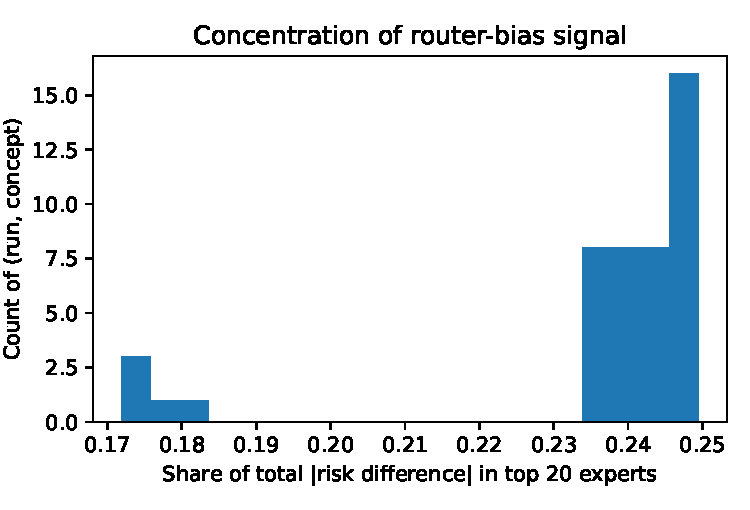
\includegraphics[width=0.7\linewidth]{expert_concentration.pdf}
  \caption{Distribution of the share of $\sum |\Delta_{\ell,e}|$ captured by
    the top $20$ $(\ell, e)$ cells, one row per (run, concept). The share is
    consistently below $0.1$, indicating a diffuse readout: there is no small
    set of experts that explains most of the prefix-conditioned vs.\
    unprefixed routing-rate gap on \mixtral.}
  \label{fig:expert_concentration}
\end{figure}

This matters mechanistically. \steermoe~works as advertised when there is a
small $(\ell, e)$ subset whose activation rate differs sharply between
contrastive prompt sets, because the additive bias on those few experts
suffices to redirect routing. When the differential signal is diffuse, the
sparse top-$k$ plan amounts to a small bias on a small number of cells out
of $L \cdot E = 32 \cdot 8 = 256$, which is unlikely to dominate the
unbiased router logit distribution at decode time.

\paragraph{Steering-strength sweep.}
Figure~\ref{fig:steering_strength} plots mean response length against the
steering coefficient for the question-only ablations. The qualitative pattern
matches Claim~2: the baseline curve is essentially flat across configurations,
and the SteerMoE curve drops monotonically as $\alpha$ grows, but neither
curve interacts with concept-token hits in any visible way. (We report
length here because it is the only diagnostic that moves smoothly with
$\alpha$.)

\begin{figure}[ht]
  \centering
  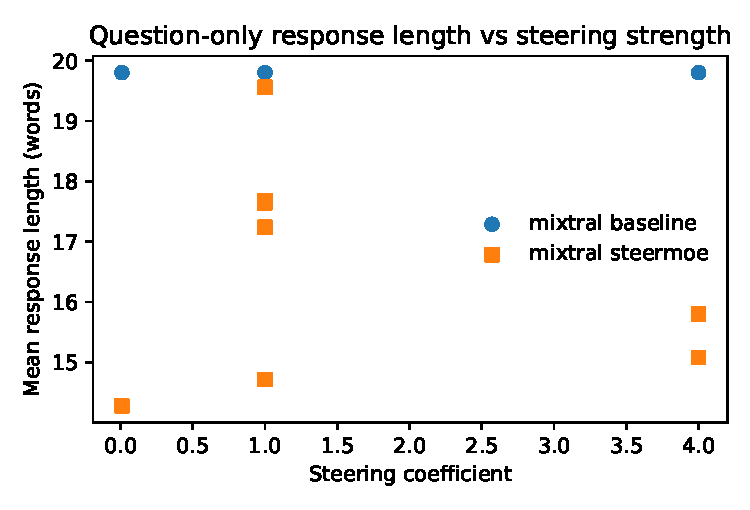
\includegraphics[width=0.7\linewidth]{steering_strength_sweep.pdf}
  \caption{Mean response length (words) vs steering coefficient under the
    question-only contract. Baseline is flat, \steermoe~contracts response
    length as $\alpha$ grows but does not produce a corresponding rise in
    the concept-token hit rate.}
  \label{fig:steering_strength}
\end{figure}

\subsection{What this leaves on the table}
\label{sec:results-discussion}

We read the three claims together as: \steermoe~as written transfers a
small, mostly-defocusing signal to \mixtral~under a question-only test on
fear concepts. There are at least three plausible reasons consistent with
this picture:

\begin{enumerate}
  \item \textbf{Readout is too crude.} The matched-target-span readout
  averages over every token in the shared statement body. If the
  concept-distinctive routing pattern is concentrated in a few attended
  positions, averaging dilutes it. This is the prediction
  attention-guided steering~\citep{tan2024attentionguided} is designed to
  improve.
  \item \textbf{Intervention site is wrong.} Hidden-state activation
  steering on the residual stream might be cleaner than router-logit
  steering on a model where the differential signal is diffuse across
  experts. The same upstream attention-guided readout would also feed
  hidden-state steering naturally.
  \item \textbf{Concept family is too abstract.} Fear is not a syntactic
  category and need not produce a sharp router signature on Mixtral. A
  more lexical concept family --- e.g., a political-figure family --- might
  produce a more concentrated risk-difference table.
\end{enumerate}

The follow-up experiment that distinguishes (1) and (2) from (3) is
described in Section~\ref{sec:conclusion}.

\section{Discussion and Future Work}
\label{sec:conclusion}

The headline of this paper is intentionally narrow. We re-implemented
\steermoe~close to the upstream paper, applied it to \mixtral~on a
question-only fear-concept test, swept the natural knobs, and observed
small, mostly-defocusing shifts rather than concept-specific transfer.
The risk-difference signal that drives the steering plan is diffuse on
\mixtral, which is consistent with the question-only behavior.

\paragraph{What this is, and is not, evidence for.}
We are not claiming \steermoe~is broken. The original demonstration uses
different MoE checkpoints, different prompt families, and a different
test contract. We are claiming that on the specific transfer setup we
ran --- \mixtral, fear concepts, question-only test --- the upstream
recipe is not enough on its own. That is a useful diagnostic both for
practitioners considering routing-bias steering on Mixtral-class models
and for follow-up work that wants to compare readout rules at fixed
intervention site.

\paragraph{Same-data, same-model method comparison.}
The natural follow-up is a same-Mixtral, same-data comparison of three
columns:

\begin{enumerate}
  \item \mixtral~baseline,
  \item \mixtral~+ attention-guided activation steering on hidden states,
  \item \mixtral~+~\steermoe~(this paper's setup).
\end{enumerate}

This is the experiment our codebase is staged for. The
attention-collection scaffolding under
\texttt{collect\_attention\_to\_prefix.py} and
\texttt{src/.../attention\_collection.py} already produces the
attention-to-prefix tensors that an attention-guided readout requires;
what is missing is the hidden-state readout-and-edit backend that turns
those tensors into a steering plan. Adding that backend without
changing the dataset, the prompt contracts, or the report schema is a
deliberate design choice of the current repo.

\paragraph{Concept-family generalization.}
A second axis we did not explore is whether the diffuse-signal finding
holds on more lexical concept families. If a political-figure or
profession concept family produces a sharply concentrated
risk-difference table on the same Mixtral checkpoint, the diffuse-signal
explanation would localize to the fear-concept setting rather than to
\mixtral. This would shift the implication of Claim~3 from
``\steermoe-on-\mixtral~needs a better readout'' toward
``\steermoe-on-\mixtral~needs a more lexical target concept''. We
consider both worth running before any method-comparison conclusion.

\paragraph{What we will and will not try to claim later.}
The codebase keeps the model-specific and method-specific pieces
deliberately separated --- \texttt{mixtral\_backend.py} is the active
router-tracing layer, \texttt{olmoe\_backend.py} is the previous
implementation we used to validate the readout shape, and the
attention-collection module is shared. That separation is what lets
this paper make a narrow Claim~2/3 about \steermoe-on-\mixtral~without
overcommitting to a method comparison the data cannot yet support.
The next paper, if the planned method comparison comes through, will
have to be more ambitious; this one does not.

\section{Broader Impact}
\label{sec:broader_impact}

This paper studies a steering technique on a frozen open-weight model. It
neither produces a new model checkpoint nor a new training procedure. The
direct uplift to a malicious actor from a successful steering technique on
fear concepts is small relative to existing prompt-based jailbreaks: the
technique reported here demonstrably does not produce concept-specific
shifts, and the question-only test contract is more constrained than
arbitrary user input.

The methodological contribution we do see is honest: studies that
re-implement and stress-test recently-proposed interventions on
publicly-available checkpoints help calibrate the field's expectations
about which methods transfer and which were checkpoint-specific. We
strongly prefer this kind of small, narrow, conservative-claim study
over headline benchmarks that report only the configurations on which
the method works. We follow the upstream community norm of making the
prompts, generation metadata, and aggregation scripts open under the
same license as the codebase.

A residual concern is that any successful steering method --- including
one that improves on the result reported here --- could in principle
be repurposed to bias model output toward content the model would
ordinarily avoid. We do not pursue that direction in this paper, and
the codebase does not include adversarial-prompt datasets. Future
extensions that compare attention-guided activation steering against
\steermoe~on the same checkpoint should explicitly evaluate against
the safety filters of the deployed model rather than only against
neutral concept families.

\section*{Acknowledgements}

Compute for the \mixtral~runs was provided by Harvard ORCD's
\texttt{mit\_normal\_gpu} partition. Code review and discussion of the
\steermoe~readout target span benefited from collaborator feedback;
remaining errors are mine. The fear-concept dataset and evaluation
prompts are adapted from the upstream activation-steering literature
referenced in the codebase under
\texttt{docs/UPSTREAM\_DATA.md}.


\bibliographystyle{plainnat}
\bibliography{references}

\appendix
\section{Run inventory}
\label{app:runs}

The aggregated tables and figures in Section~\ref{sec:results} were derived
from the following committed runs under \texttt{experiments/}:

\begin{itemize}
  \item \texttt{prefix\_conditioned\_model\_comparison\_fears\_seed7\_mixtral\_8bit}
  -- Stage 1, full-prefix comparison across \llama, \olmoe, \mixtral.
  \item \texttt{mixtral\_steermoe\_fears\_seed7\_question\_only\_with\_llama}
  -- Stage 2 main run; the Llama-reference column is unsteered.
  \item \texttt{mixtral\_steermoe\_fears\_seed7\_question\_only\_coef1\_pos8\_neg0},
        \texttt{coef1\_pos20\_neg0}, \texttt{coef1\_pos10\_neg100},
        \texttt{coef4\_pos8\_neg0}, \texttt{coef4\_pos8\_neg8} --
        steering-knob ablations under the question-only contract.
  \item \texttt{mixtral\_steermoe\_fears\_seed7\_question\_only\_paper\_eps001\_pos20\_neg0},
        \texttt{prefix\_conditioned\_paper\_eps001\_pos20\_neg0} --
        paper-rule sanity runs at the original threshold and selection counts.
  \item \texttt{olmoe\_steermoe\_fears\_seed7\_question\_only} -- earlier
        OLMoE implementation kept as a reference for the readout shape.
\end{itemize}

\section{Reproducing the tables}
\label{app:repro}

The aggregation pipeline does not require model weights. From a clean
checkout:

\begin{verbatim}
python3 paper/scripts/aggregate_results.py
python3 paper/scripts/make_figures.py
\end{verbatim}

The first script walks \texttt{experiments/} and writes
\texttt{paper/notebooks/sweep\_results.csv} (one row per (run, response))
and \texttt{paper/notebooks/expert\_selection.csv} (one row per
(run, layer, expert)). The second script reads those CSVs and writes the
LaTeX tables and PDF figures under
\texttt{paper/docs/paper/tables/} and \texttt{paper/docs/paper/figures/}.

\section{Decoding configuration}
\label{app:decoding}

All generation calls use:

\begin{itemize}
  \item temperature $0$, top-$p$ $1.0$,
  \item \texttt{max\_new\_tokens} $= 48$,
  \item the chat template shipped with each model's tokenizer,
  \item per-model load precision: \mixtral~8-bit (\texttt{bitsandbytes}
  with CPU offload), \llama~16-bit, \olmoe~16-bit.
\end{itemize}

\section{Selected steering plans}
\label{app:plans}

For reference, each run's per-concept steering plan is checked in under
\texttt{experiments/<run\_dir>/steering\_plans/}. Each plan file lists
the selected $(\text{layer}, \text{expert}, \text{sign})$ tuples and the
risk-difference value at the time of selection. Plans are derived from
the activation tables under \texttt{activation\_tables/} in the same
run directory.


\end{document}
